\documentclass[12pt,onecolumn]{article}
\usepackage[utf8]{inputenc} % UTF8 input encoding
\usepackage[T2A]{fontenc}   % T2A font encoding for Cyrillic script
\usepackage[russian]{babel} % Russian language support
\usepackage{listings}
\usepackage{float}
\usepackage{mathtools}
\usepackage{longtable}
\everymath{\displaystyle}
\usepackage{listings} 
\usepackage[usenames]{color}
\usepackage{geometry}
\usepackage{verbatim}
\geometry{
  a4paper,
  top=25mm, 
  right=15mm, 
  bottom=25mm, 
  left=15mm
}

\begin{document}
\setcounter{tocdepth}{4}
\begin{center}
    Федеральное государственное автономное образовательное учреждение высшего образования "Национальный Исследовательский Университет ИТМО"\\ 
    Мегафакультет Компьютерных Технологий и Управления\\
    Факультет Программной Инженерии и Компьютерной Техники \\
    
\includegraphics[scale=0.3]{image/itmo.jpg} % нужно закинуть картинку логтипа в папку с отчетом
\end{center}
\vspace{1cm}


\begin{center}
    \textbf{Курсовая работа этап 2}\\
    по дисциплине\\
    \textbf{'Информационные системы и базы данных'}\\
\end{center}

\vspace{2cm}

\begin{flushright}
  Выполнили Студенты  группы P33102\\
  \textbf{Лапин Алексей Александрович}\\
  \textbf{Юнусов Роман Ильдарович}\\
  Преподаватель: \\
  \textbf{Сагайдак Алина Алексеевна}\\
\end{flushright}

\vspace{6cm}
\begin{center}
    г. Санкт-Петербург\\
    2023г.
\end{center}

\newpage
\tableofcontents
\newpage
\section{Текст задания.}
\begin{itemize}
  \item Нарисовать ER-диаграмму предметной области. ER-модель должна соответствовать
  описанию, представленному в рамках первого этапа курсовой работы.
  \item На основе ER-модели построить даталогическую модель.
\end{itemize}
\subparagraph{Требования к ER-модели и БД:}
\begin{itemize}
  \item ER-модель должна соответствовать представленному описанию предметной области.
  \item ER-модель базы данных должна включать в себя не менее 10 сущностей, содержать
  хотя бы одно отношение «многие-ко-многим».
  \item В качестве СУБД должна использоваться СУБД PostgreSQL. Для реализации БД и
  вспомогательных средств должны использоваться языки SQL и PL/pgSQL База данных
  должна быть развернута на сервере helios.
  \item Веб-приложение, использующее разработанную базу данных, должно быть развернуто
  на сервере helios.
  \item Взаимодействие с БД/запуски запросов и скриптов должны осуществляться через psql.
\end{itemize}
\section{Описание предметной области.}
Магазин покемонов.\\
Существуют тренеры и покемоны. В нашем магазине продаются покемоны и камни эволюции. Наш магазин умеет предлагать к покупке покемонов соответствующие уровню и стилю игры тренера. Некоторые из покемонов могу эволюционировать в других покемонов при применении подходящего камня эволюции. 
\section{ER-модель.}
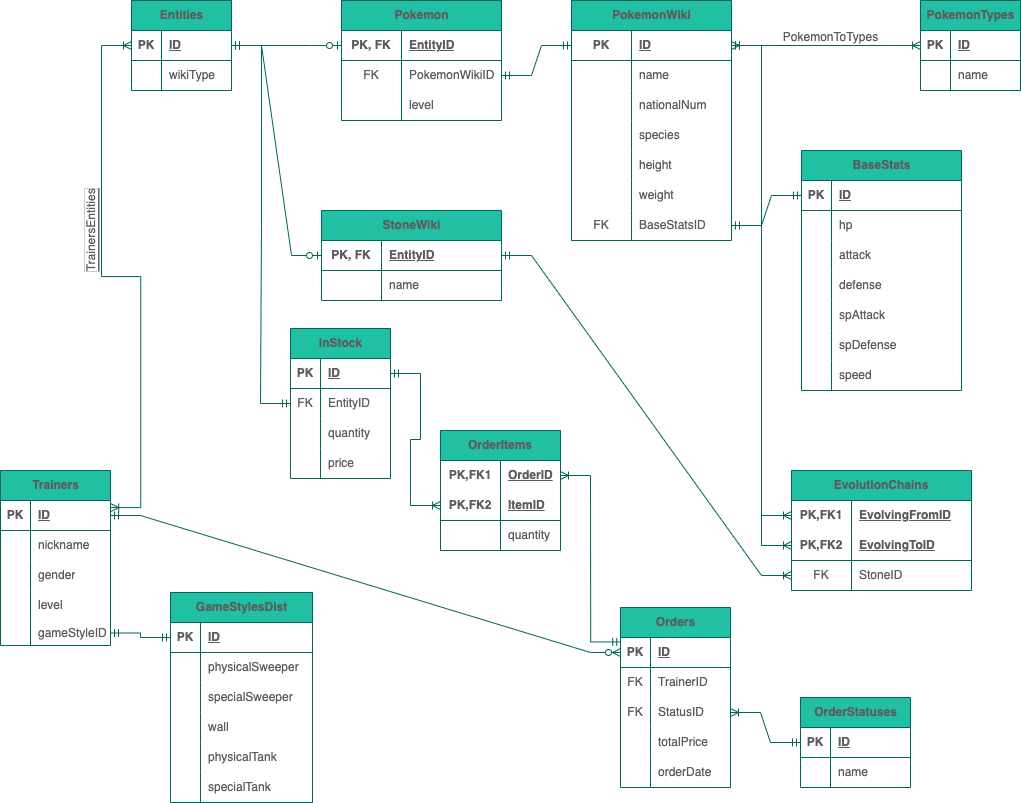
\includegraphics[width=\textwidth]{image/infological-model.png}
\section{Даталогическая модель.}
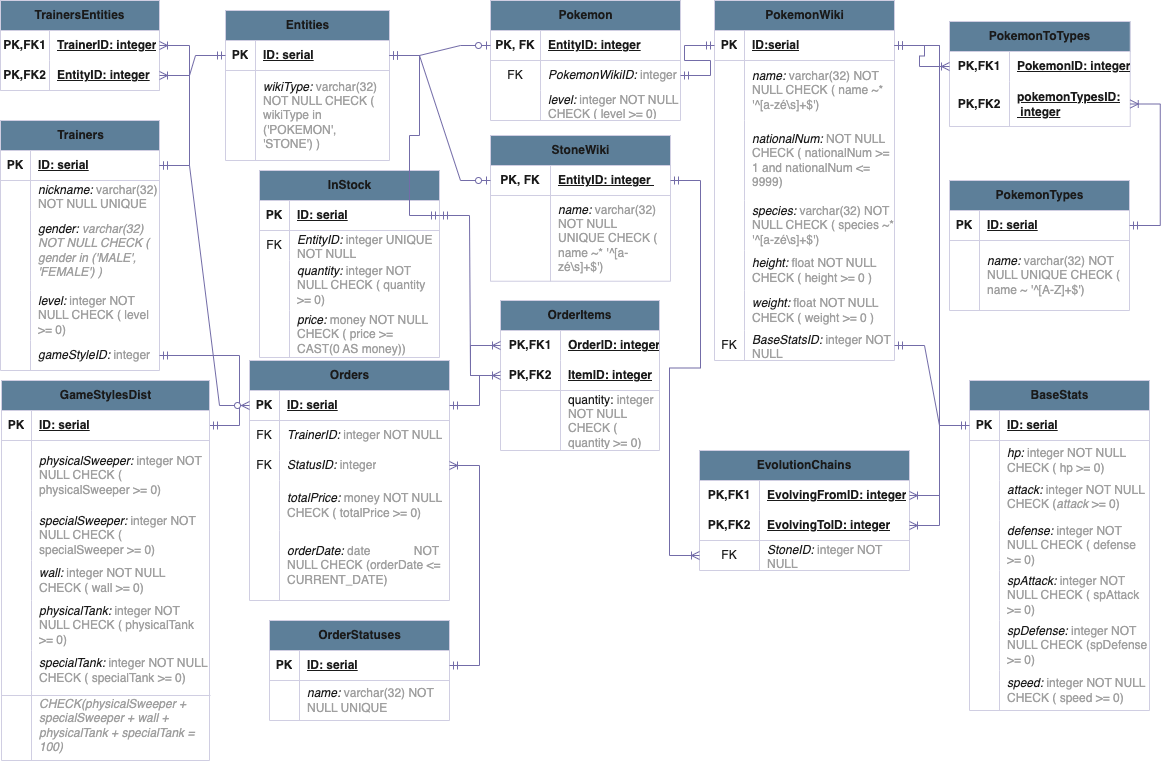
\includegraphics[width=\textwidth]{image/datalogical-model.png}
\end{document}